\subsection[Algoritmi Ensemble]{\textit{Algoritmi Ensemble}}

%\subsubsection[Training e test set]{Training e test set}

\begin{frame}
	
	\frametitle{Algoritmi Ensemble}
	
	\begin{figure}[!htbp]
		\centering
		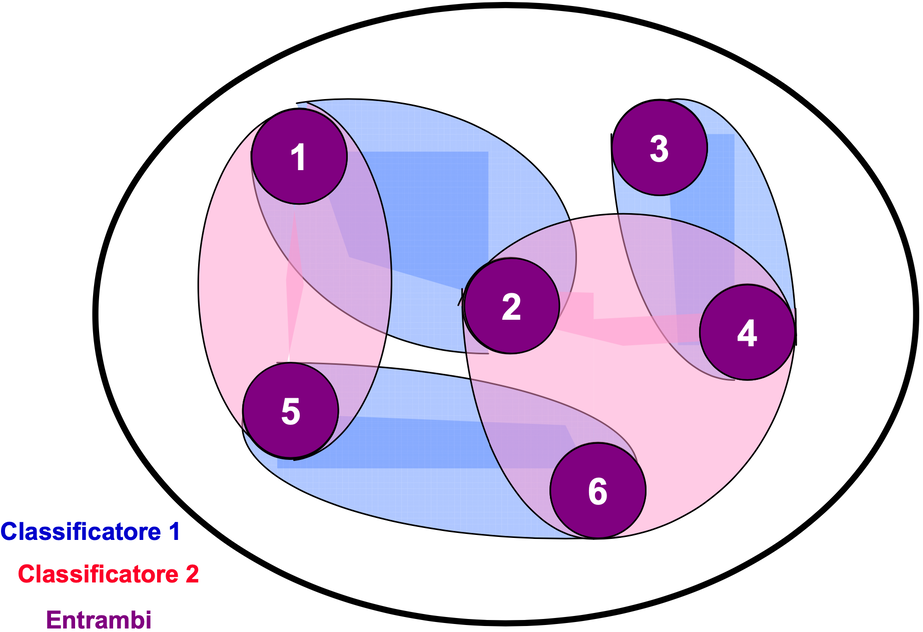
\includegraphics[width=0.90\linewidth]{images/supervised/z_algorithms_ensemble/ensemble.png}
		%\caption{}
	\end{figure}
	 
\end{frame}

\begin{frame}
	
	\frametitle{Algoritmi Ensemble}
	
	Dopo aver scoperto tanti algoritmi complessi e potenti, potreste rimanere sorpresi dal fatto che una \textbf{sommatoria di algoritmi} di machine learning più semplici \textbf{può avere prestazioni molto migliori} di quelle di singoli algoritmi più sofisticati.
	\newlinedouble
	Questa è appunto la \textbf{potenza degli ensemble}, gruppi di modelli che lavorano insieme per produrre previsioni migliori. La cosa stupefacente degli ensemble è che sono costituiti da gruppi di algoritmi che, singolarmente, non hanno grandi prestazioni.
	\newlinedouble
	Gli ensemble funzionano in modo non dissimile dall'\textbf{intelligenza collettiva delle folle}: in pratica, facendo la media di un insieme di risposte errate, si ottiene la risposta corretta.
	
%	\begin{figure}[!htbp]
%		\centering
%		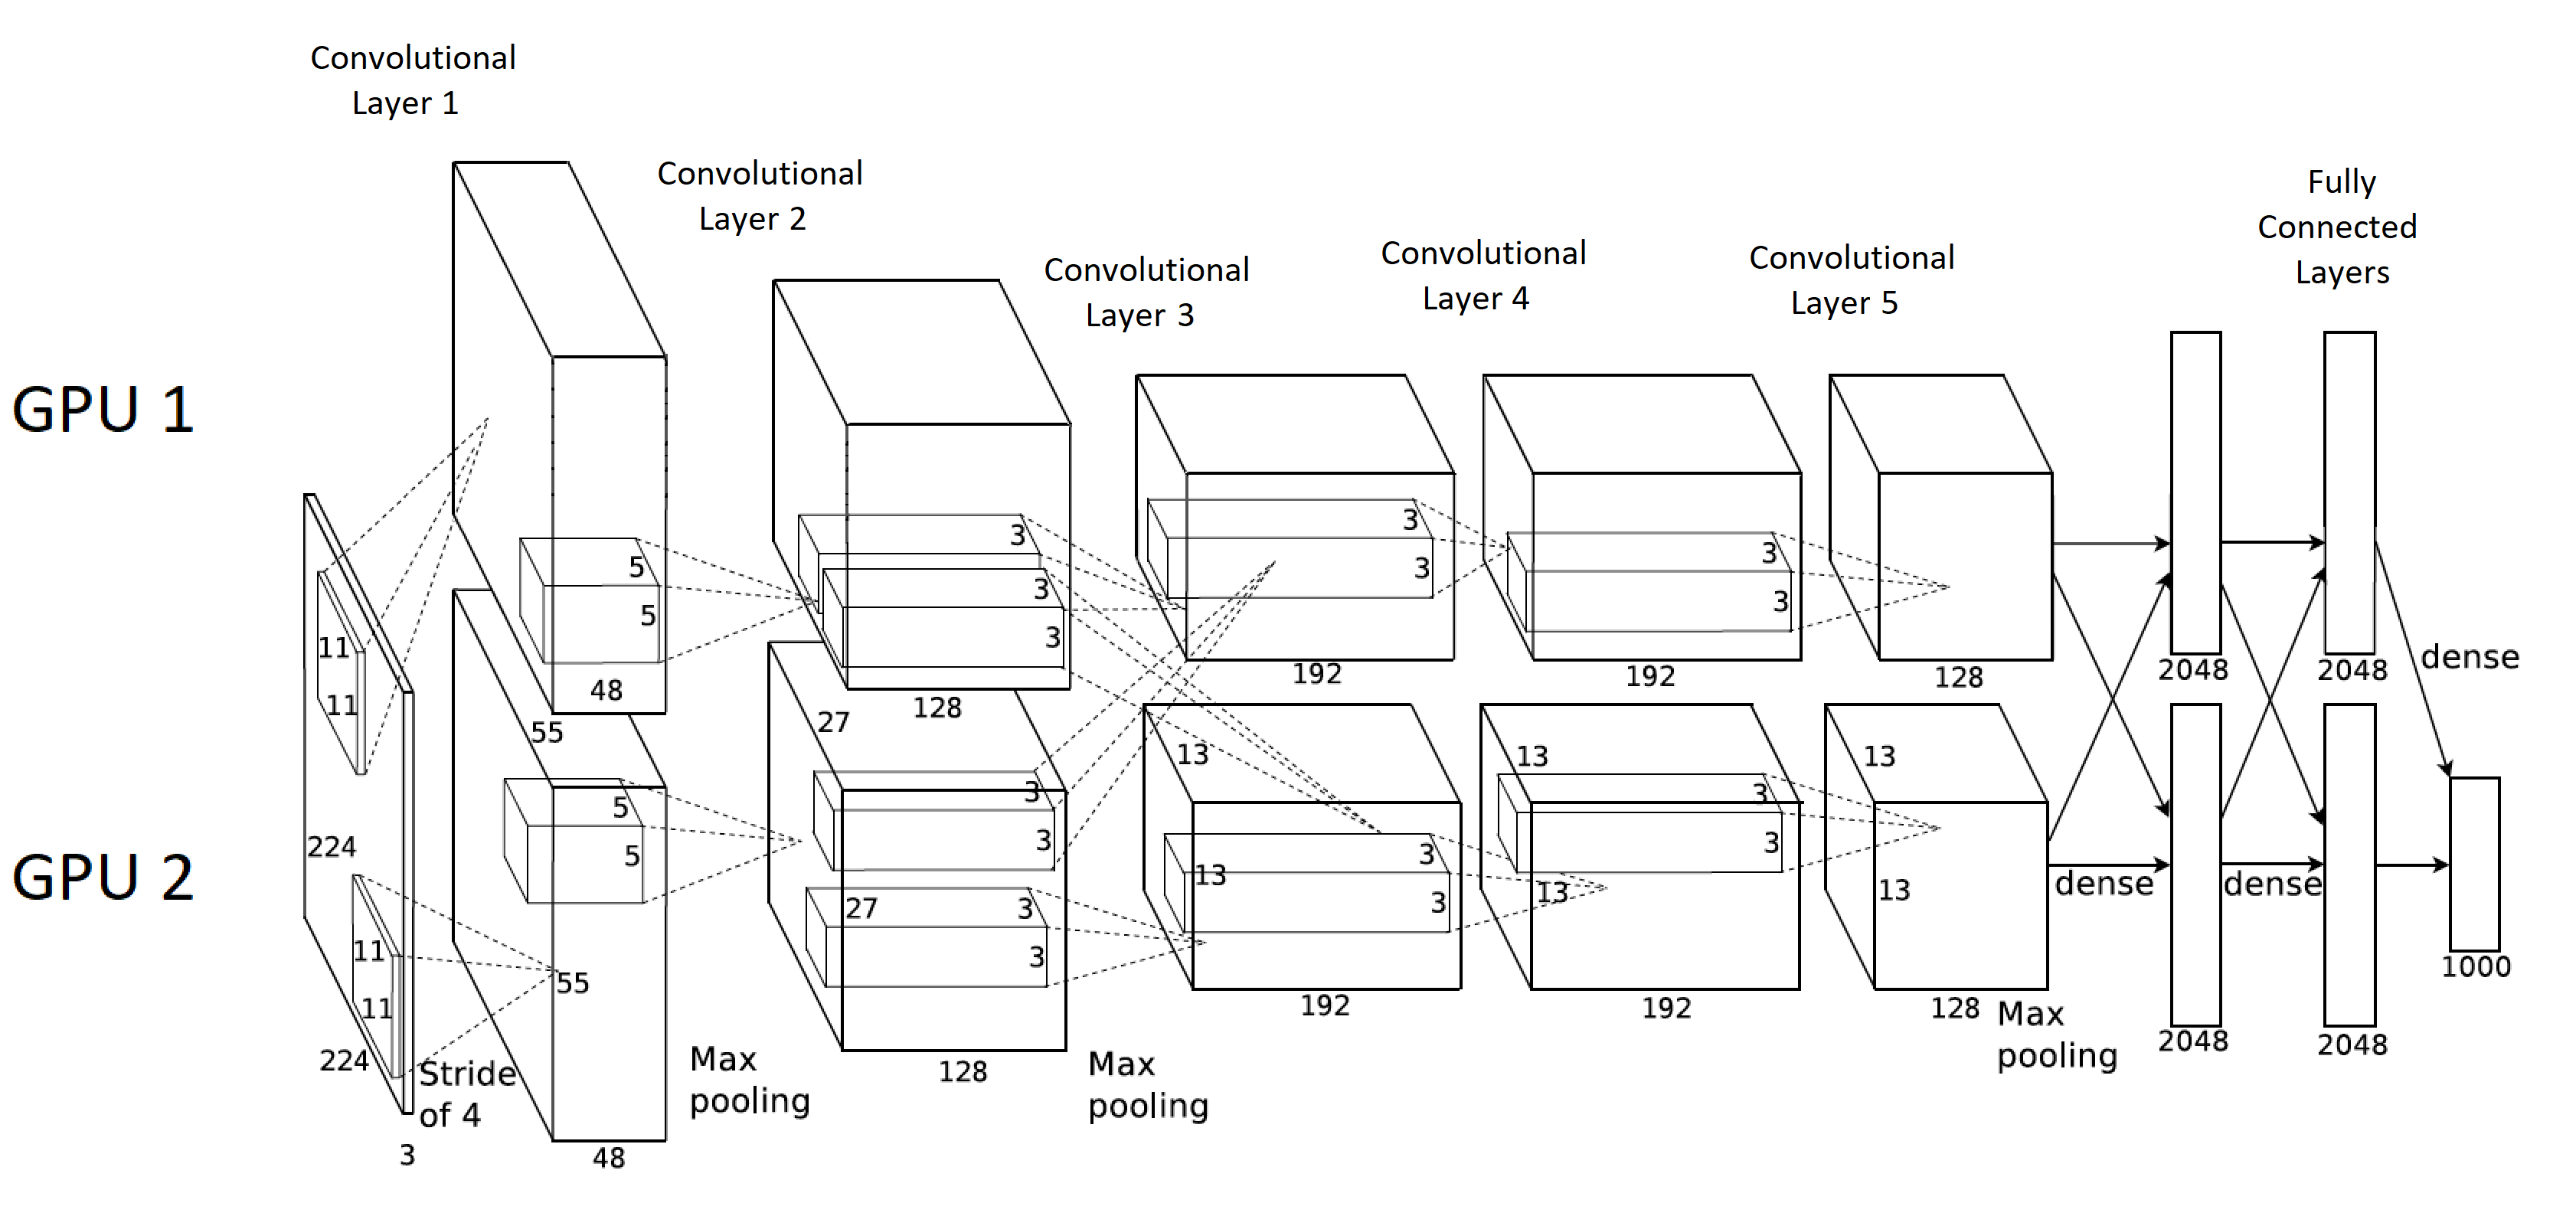
\includegraphics[width=1.0\linewidth]{images/supervised/z_algorithms_deep_learning/tensor_1.png}
%		%\caption{}
%	\end{figure}	

\end{frame}


\begin{frame}
	
	\frametitle{Algoritmi Ensemble}
	
	
	\begin{columns}
		\column{0.55\linewidth}	
		Sir Francis Galton, lo statistico dell'era vittoriana, raccontava \textbf{l'aneddoto di una folla} che, in una festa paesana, riusciva ad indovinare il peso corretto di un bue dopo aver fatto la media delle precedenti risposte di tutte le persone che avevano già provato a indovinarne il peso.
		\newlinedouble
		Dietro i risultati non c'è la fortuna: semplicemente, è in funzione la \textbf{legge dei grandi numeri}.\\
		Anche se il singolo individuo ha scarse probabilità di trovare la risposta giusta, la congettura risulta migliore rispetto a un valore casuale.
		
		\column{0.45\linewidth}
		\begin{figure}[!htbp]
			\centering
			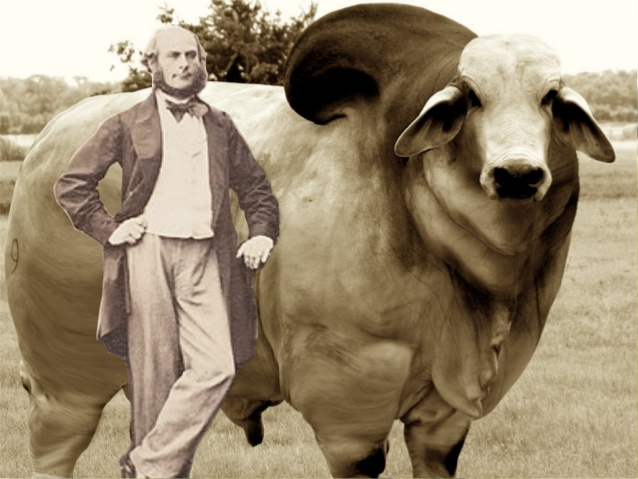
\includegraphics[width=0.9\linewidth]{images/supervised/z_algorithms_ensemble/weight_guessing_competition_1.jpg}
			%\caption{}
		\end{figure}
		
		\begin{figure}[!htbp]
			\centering
			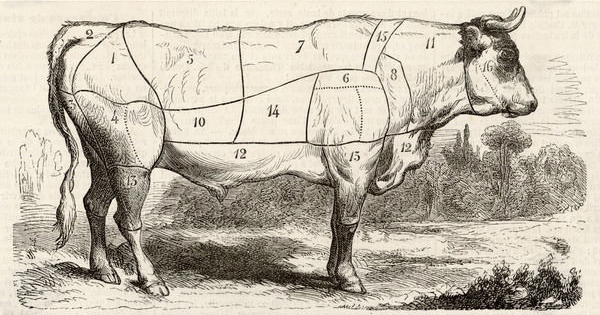
\includegraphics[width=0.9\linewidth]{images/supervised/z_algorithms_ensemble/weight_guessing_competition_2.jpg}
			%\caption{}
		\end{figure}
	\end{columns}

	
%	\begin{figure}[!htbp]
%		\centering
%		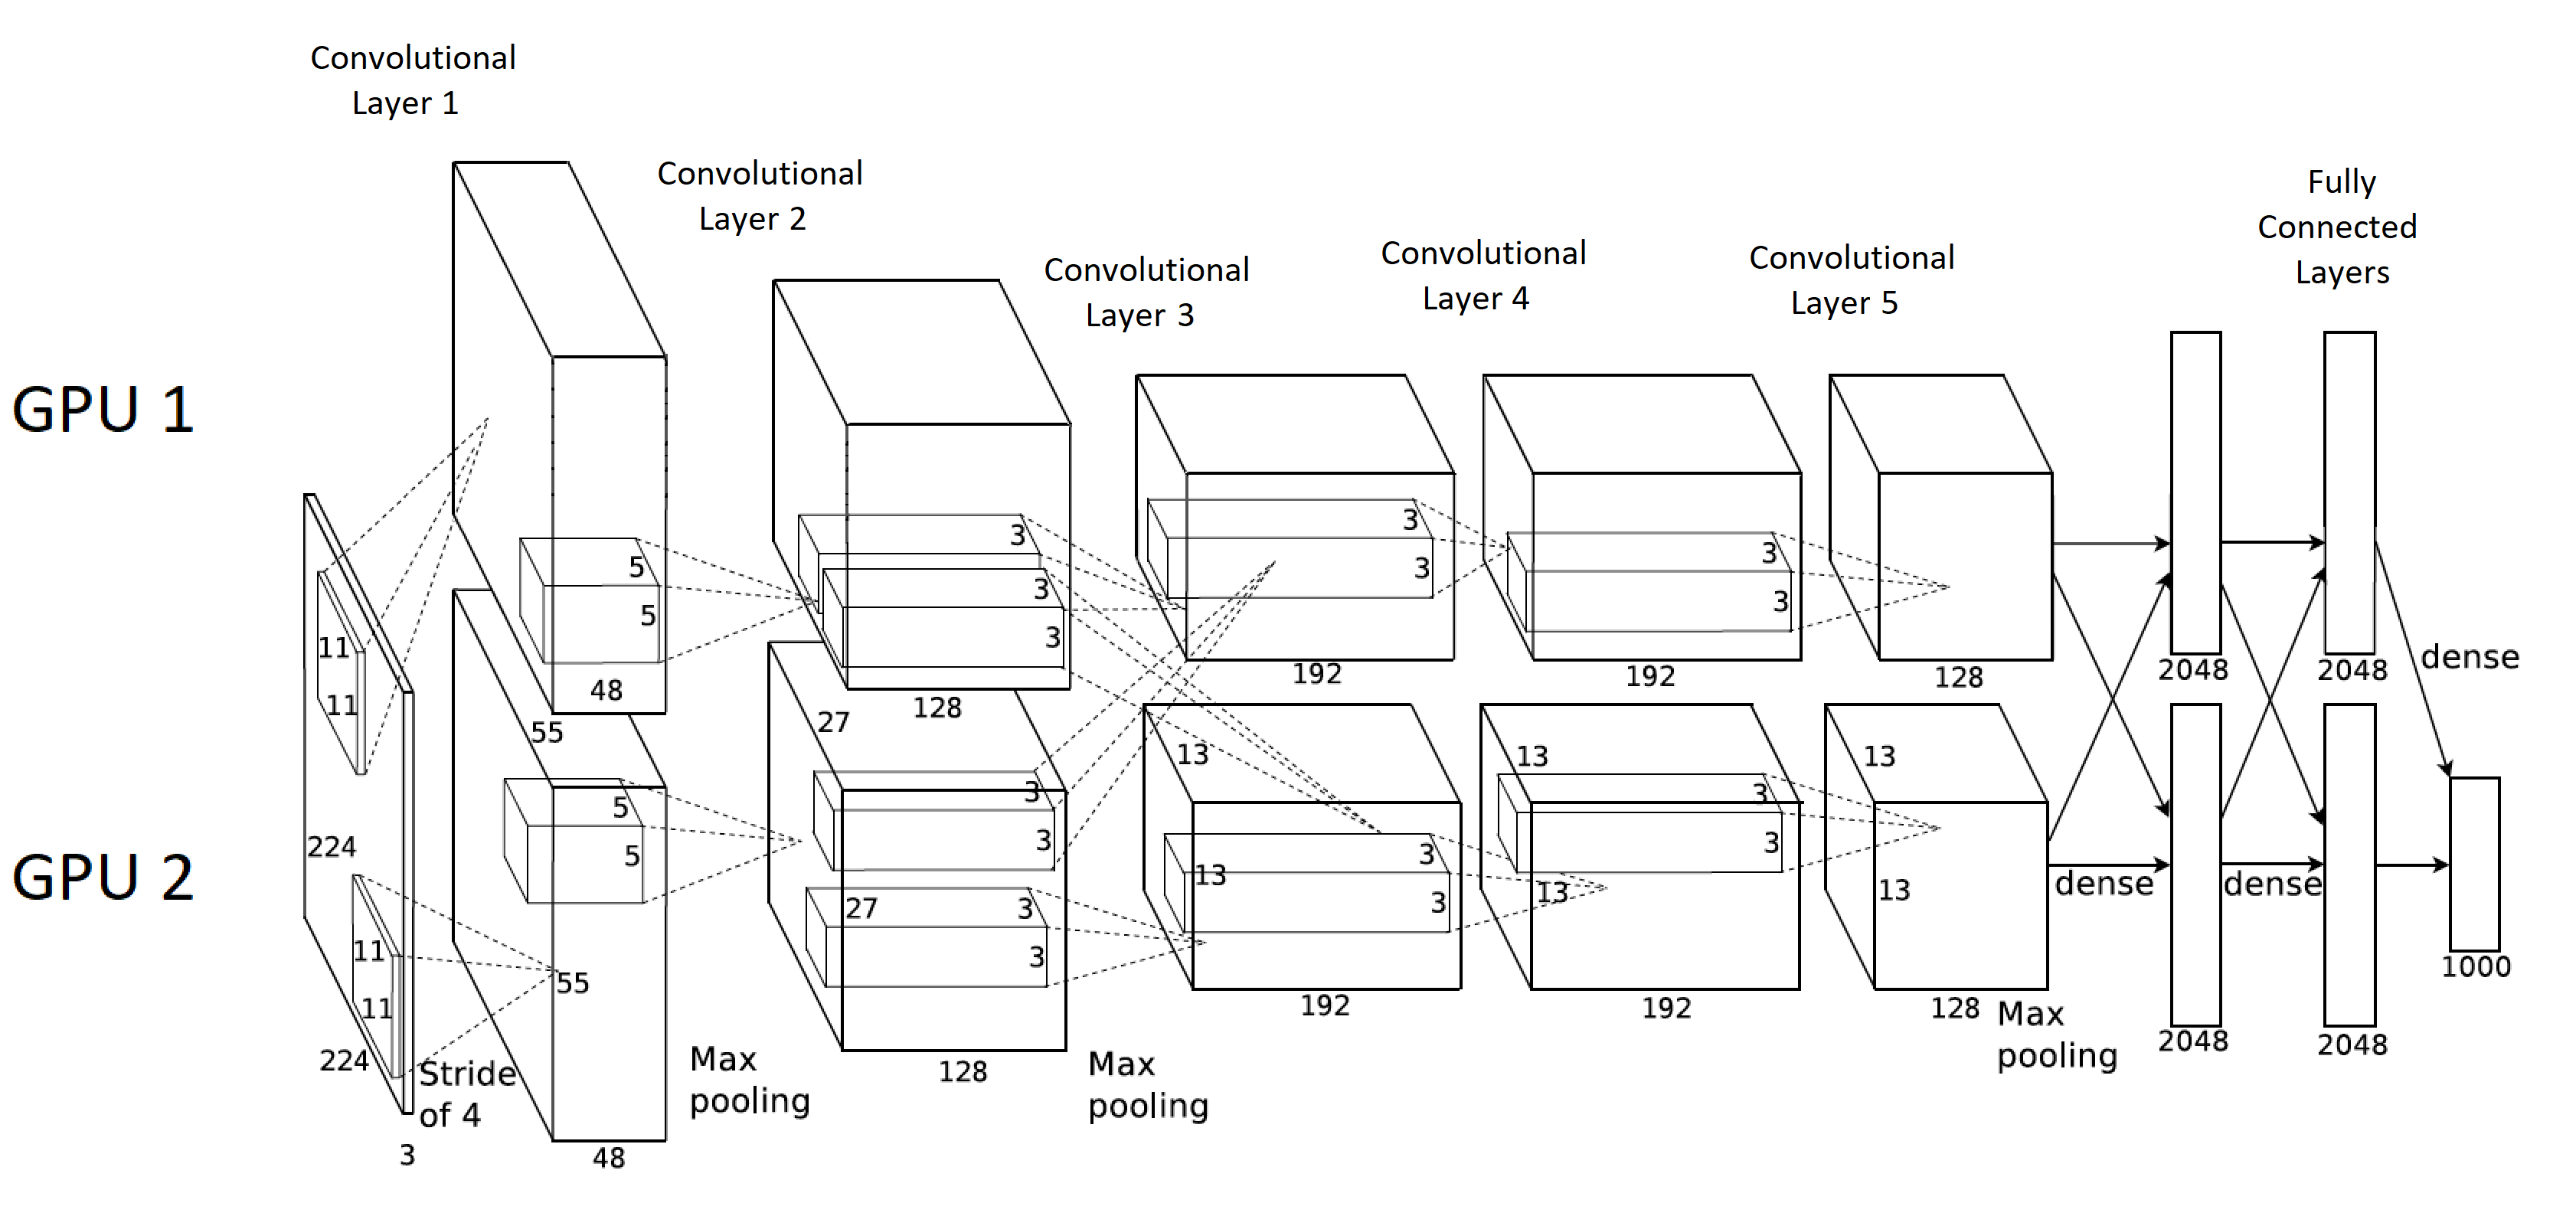
\includegraphics[width=1.0\linewidth]{images/supervised/z_algorithms_deep_learning/tensor_1.png}
%		%\caption{}
%	\end{figure}	

\end{frame}


\begin{frame}

	\frametitle{Algoritmi Ensemble: applicati agli alberi di decisione}

	\begin{figure}[!htbp]
		\centering
		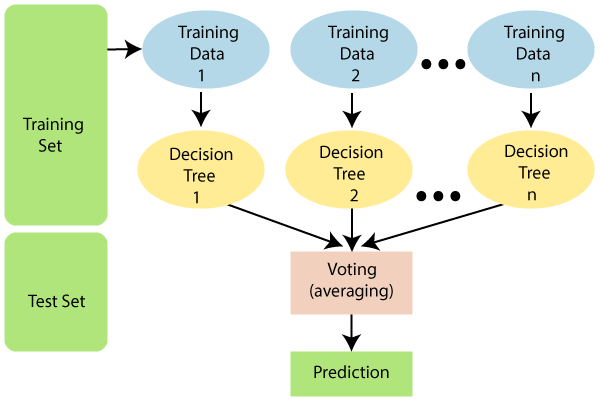
\includegraphics[width=0.8\linewidth]{images/supervised/z_algorithms_ensemble/random_forest_algorithm_1.png}
%			\caption{}
	\end{figure}

\end{frame}


\begin{frame}

	\frametitle{Algoritmi Ensemble: applicati agli alberi di decisione}

	\begin{figure}[!htbp]
		\centering
		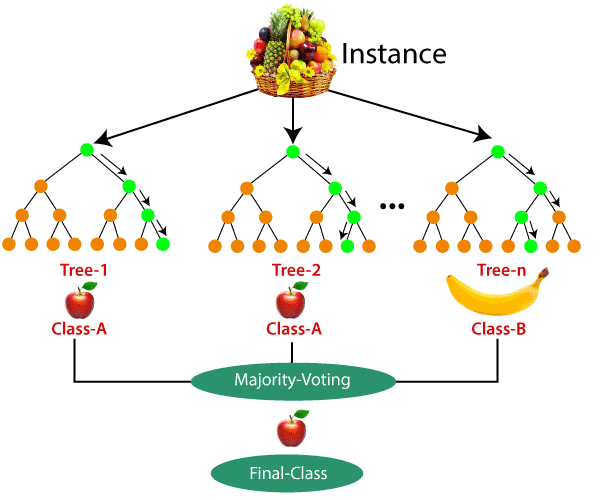
\includegraphics[width=0.7\linewidth]{images/supervised/z_algorithms_ensemble/random_forest_algorithm_2.png}
%			\caption{}
	\end{figure}

\end{frame}


\subsubsection[Bagging]{\textit{Bagging}}
\begin{frame}
	\frametitle{Bagging}
	
	\begin{itemize}
		\item Il \textbf{bagging} (da \textbf{b}ootstrap \textbf{agg}regat\textbf{ing}) è una procedura generale per ridurre la varianza di una tecnica di apprendimento statistico
		\item Idea: Se $Z_1,Z_2,\ldots,Z_n$ sono estrazioni IID da $D(\mu,\sigma^2)$, allora 
		\[
		\E(\overline Z) = \mu \quad \mbox{e} \quad \Var(\overline Z) = \frac{\sigma^2}{n}
		\]
		Calcolare la media permette di ridurre la varianza
		\item Per calcolare la media su più stime ci servono più campioni di addestramento. Dove li troviamo?
		\item \emph{Usiamo il bootstrap}: estraiamo campioni dal dataset originario
	\end{itemize}
\end{frame}
	
	
\begin{frame}
	\frametitle{Algoritmo bagging}
	
	\begin{itemize}
		\item Supponiamo di voler costruire un predittore bagging in $X=x$
		\item Generiamo $B$ campioni di addestramento diversi usando il bootstrap
		\item Addestriamo il metodo su ogni campione di addestramento generato con il bootstrap
		\item Otteniamo $\widehat f_b^*(x)$, $b=1,2,\ldots,B$
			\begin{itemize}
				\item in un problema di regressione, calcoliamo la media delle previsioni:
				\[
				\widehat f_{bag}(x) = \frac{1}{B} \sum_{b=1}^B \widehat f_b^*(x)
				\]
				
				\item in un problema di classificazione, usiamo la \emph{regola della maggioranza}, oppure classifichiamo usando la probabilità media prevista
			\end{itemize}
	\end{itemize}
\end{frame}


\begin{frame}
	\frametitle{Errore OOB}
	
	\begin{itemize}
		\item Il bagging è particolarmente efficace quand'è usato sugli alberi
		%\item Con il bagging, gli alberi non devono necessariamente essere potati; il bagging provvede a ridurre la varianza elevata del metodo
		\item Valori elevati di $B$ non generano \emph{overfitting}, ma il loro contributo marginale è decrescente
		\item L'errore \emph{Out-Of-Bag} (OOB) semplifica la stima dell'errore di test di un modello addestrato con il bagging
		\begin{itemize}
			\item in media, ogni albero del bagging usa 2/3 delle $n$ osservazioni
			\item il 1/3 rimanente contiene le cosiddette osservazioni \emph{out of bag, OOB}
			\item per ciascuno degli alberi in cui l'osservazione $i$-esima era OOB, prevediamo $y_i$
			\item calcoliamo la media o calcoliamo la maggioranza delle (approssimativamente) $B/3$ risposte previste
			\item usiamo queste previsioni per calcolare l'EQM  e l'errore di classificazione OOB
			\item Per $B$ elevati, OOB è molto vicino a LOOCV
		\end{itemize}
	\end{itemize}
\end{frame}


\subsubsection[Random Forests (RF)]{\textit{Random Forests (RF)}}
\begin{frame}
	\frametitle{Foreste casuali (\emph{Random forests, RF})}
	
	\begin{itemize}
		\item Nel bagging, i campioni generati con il bootstrap sono \emph{correlati} % (nonché gli alberi e i predittori basati su di essi)
		\item La procedura RF rappresenta un miglioramento rispetto al bagging perché genera alberi \emph{meno correlati}
		\item Come il bagging, RF agisce su $B$ campioni generati dal bootstrap
		\item Per ogni dataset $b$, ad ogni passo della procedura di costruzione dell'albero \emph{consideriamo solo $m<p$ covariate scelte in maniera casuale}. Di solito:
		    \begin{itemize}
			    \item $m=\sqrt{p}$ per problemi di classificazione
			    \item $m=p/3$ per problemi di regressione
			    \item ($m=p$ corrisponde al bagging descritto nelle slide precedenti)
		    \end{itemize}
		\item Nell'algoritmo RF, gli alberi sono \emph{costretti} a essere diversi, riducendo la correlazione
		\item Come nel bagging:
			\begin{itemize}
				\item un $B$ elevato non genera overfitting, ma il contributo marginale di un campione bootstrap aggiuntivo è decrescente
				\item l'errore \emph{Out-Of-Bag} (OOB) semplifica la stima dell'errore di test
			\end{itemize}
	\end{itemize}
\end{frame}


\begin{frame}
	\frametitle{Misure di importanza delle variabili}
	
	\begin{itemize}
		\item Di solito bagging e RF sono efficaci nel migliorare la precisione delle previsioni ma complicano molto l'interpretazione del modello
			\begin{itemize}
				\item non è più possibile tracciare grafici -- abbiamo centinaia di alberi				
				\item quali sono le variabili più importanti?
			\end{itemize}
		\item Le misure di influenza relativa (\emph{Relative Influence Measures}) permettono di valutare l'importanza di ogni feature
		\item Idea:
			\begin{itemize} 
				\item per ogni $X_j$ e ogni campione generato dal bootstrap, calcoliamo la riduzione dell'EQM ottenuto dividendo rispetto alla variabile $X_j$
				\item calcoliamo la media su tutti gli alberi
			\end{itemize}
		\item Di conseguenza, ogni $X_j$ ha un \emph{punteggio}:
			\begin{itemize}
				\item se è vicino a zero, $X_j$ non è molto importante
				\item se è elevato, $X_j$ è molto importante
			\end{itemize}
		\item Di solito questi punteggi sono rappresentati graficamente usando un istogramma
	\end{itemize}
\end{frame}

\subsubsection[Boosting]{\textit{Boosting}}
\begin{frame}
	\frametitle{Boosting}
	
	\begin{itemize}
		\item Il \emph{boosting} è un approccio generale all'adddestramento di un modello di regressione o di classificazione
		\item Il boosting è basato su un'intuizione molto diversa da quella alla base del bagging o delle RF: l'\emph{addestramento lento}
		\item Indichiamo con \emph{predittore debole} (\emph{weak learner}) un predittore o classificatore molto semplice e facile da calcolare
		\item L'idea alla base del boosting è di:
			\begin{enumerate}
				\item Applicare ripetutamente il predittore debole a versioni dei dati modificati in maniera sequenziale
					\begin{itemize}
						\item sovrappesando le osservazioni difficili da prevedere o classificare
						\item sottopesare le osservazioni facili da prevedere o classificare
					\end{itemize}
				\item Per costruire la previsione finale combiniamo le previsioni di tutti i modelli stimati usando una media ponderara o sulla base della regola della maggioranza
			\end{enumerate}
	\end{itemize}
\end{frame}


\begin{frame}
	\frametitle{Algoritmo di boosting per alberi di classificazione (AdaBoost.M1)}
	
	\begin{enumerate}
		\item Fissiamo i pesi iniziali a $w_i = 1/n$, $\forall i$
		\item Per $b=1,2,\ldots,B$, ripetiamo:
			\begin{itemize}
				\item [2.1] Addestriamo un classificatore $\widehat c_b(x)$ al campione di addestramento usando i pesi $w_i$
				\item [2.2] Calcoliamo
				\[
				\epsilon_b = \frac{\sum_{i=1}^n w_i \mathbb{I}[y_i\not= \widehat c_b(x_i)]}{\sum_{i=1}^n w_i}
				\]
				\item [2.3] Calcoliamo $\alpha_b = \log[(1-\epsilon_b)/\epsilon_b]$
				\item [2.4] Aggiorniamo $w_i = w_i \exp(\alpha_b \mathbb{I}[y_i\not= \widehat c_b(x_i)])$, $i=1,2,\ldots,n$
			\end{itemize}
		\item Classifichiamo usando la media ponderata di $\widehat c_b(x)$ (chiamato \emph{classificatore boosted}):
		\[
		\widehat C_{boost}(x) = \sum_{b=1}^B \alpha_b \widehat c_b(x)
		\]
	\end{enumerate}
\end{frame}


\begin{frame}
	\frametitle{Algoritmo boosting per alberi di regressione}
	
	\begin{enumerate}
		\item Fissiamo $r_i^{(1)} = y_i$, $i=1,2,\ldots,n$
		\item Per $b=1,2,\ldots,B$, ripetiamo:
			\begin{itemize}
				\item [2.1] Addestriamo un predittore $\widehat f_b$ al campione di addestramento $(X,r^{(b)})$
				\item [2.2] Aggiorniamo i residui:
				\[
				r_i^{(b+1)} = r_i^{(b)} - \lambda \widehat f_b(x_i),\:i=1,2,\ldots,n
				\]
			\end{itemize}
		\item Calcoliamo il modello boosted:
			\[
			\widehat f_{boost}(x) = \sum_{b=1}^B \lambda \widehat f_b (x)
			\]
	\end{enumerate}
\end{frame}


\begin{frame}
	\frametitle{Discussione}
	
	\begin{itemize}
		\item Il boosting è molto efficace con gli alberi
		\item Ognuno degli alberi può essere molto piccolo, di dimensione pari a $d$ (parametro di tuning)
		\item Addestrare alberi di dimensioni ridotte su osservazioni ponderate o residui permette di migliorare lentamente $\widehat C(x)$ / $\widehat f(x)$ su osservazioni problematiche
		\item I parametri di tuning $d$ e $\lambda$ rallentano il processo, rendendo più flessibile la media ponderata
	\end{itemize}
\end{frame}


\begin{frame}
	\frametitle{Parametri di tuning per il boosting}
	
	\begin{enumerate}
		\item Il \emph{numero di alberi} $B$
			\begin{itemize}
				\item il boosting può generare overfitting se $B$ è troppo elevato, ma questo problema si presenta solo lentamente
				\item possiamo sceglierlo per CV
			\end{itemize}
		\item Il \emph{numero di suddivisioni} $d$
			\begin{itemize}
				\item una scelta frequente è $d = 1$ (l'albero è detto \emph{ceppo -- stump}). Il modello finale è additivo
				\item $d$ misura anche la \emph{profondità di interazione}, e determina il massimo ordine di interazione del modello boosted 
			\end{itemize}
		\item Il \emph{parametro di shrinkage} $\lambda$
			\begin{itemize}
				\item si tratta di un numero positivo e piccolo, di solito 0.01 o 0.001
				\item $\lambda$ controlla il tasso al quale il boosting viene addestrato
				\item un $\lambda$ molto piccolo richiede di solito un $B$ molto elevato per raggiungere un errore di testo modesto
			\end{itemize}
	\end{enumerate}
\end{frame}


\begin{frame}
	
	\frametitle{Decision Tree vs Gradient Boosting: depth 1}

	\begin{columns}
		\column{0.50\linewidth}
		\begin{figure}[!htbp]
			\centering
			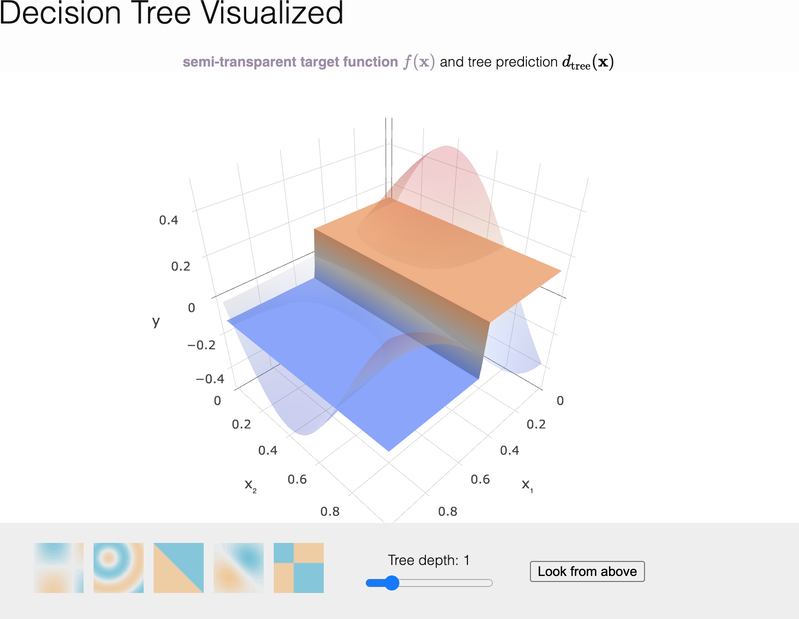
\includegraphics[width=1.0\linewidth]{images/supervised/z_algorithms_ensemble/decision_tree_depth_1.png}
%			\caption{}
		\end{figure}
		
		\column{0.50\linewidth}
		\begin{figure}[!htbp]
			\centering
			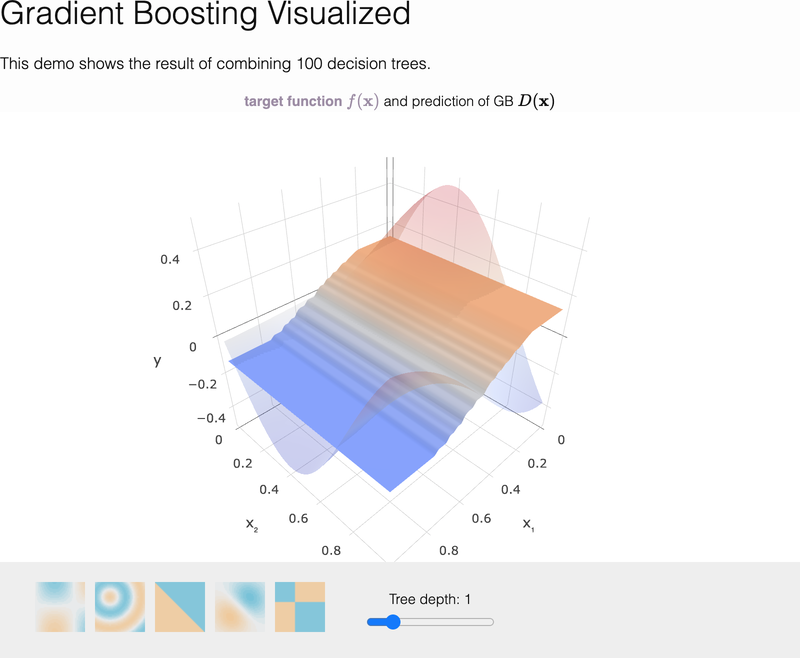
\includegraphics[width=0.93\linewidth]{images/supervised/z_algorithms_ensemble/gradient_boosting_depth_1.png}
%			\caption{}
		\end{figure}
	\end{columns}
	
	\begin{center}
		Prova la demo live al seguente link: \underline{\href{http://arogozhnikov.github.io/2016/06/24/gradient_boosting_explained.html}{Gradient Boosting explained}}
	\end{center}
	
\end{frame}


\begin{frame}
	
	\frametitle{Decision Tree vs Gradient Boosting: depth 3}

	\begin{columns}
		\column{0.50\linewidth}
		\begin{figure}[!htbp]
			\centering
			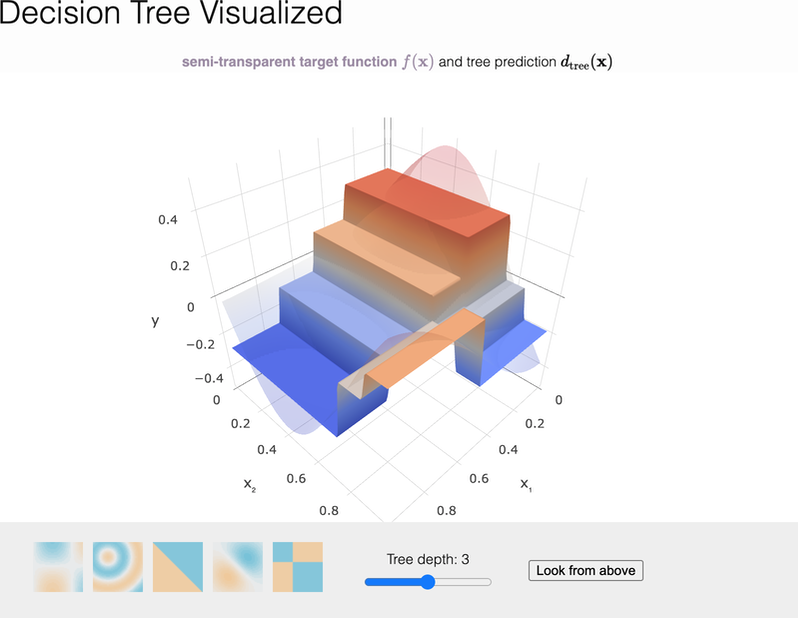
\includegraphics[width=1.0\linewidth]{images/supervised/z_algorithms_ensemble/decision_tree_depth_3.png}
%			\caption{}
		\end{figure}
		
		\column{0.50\linewidth}
		\begin{figure}[!htbp]
			\centering
			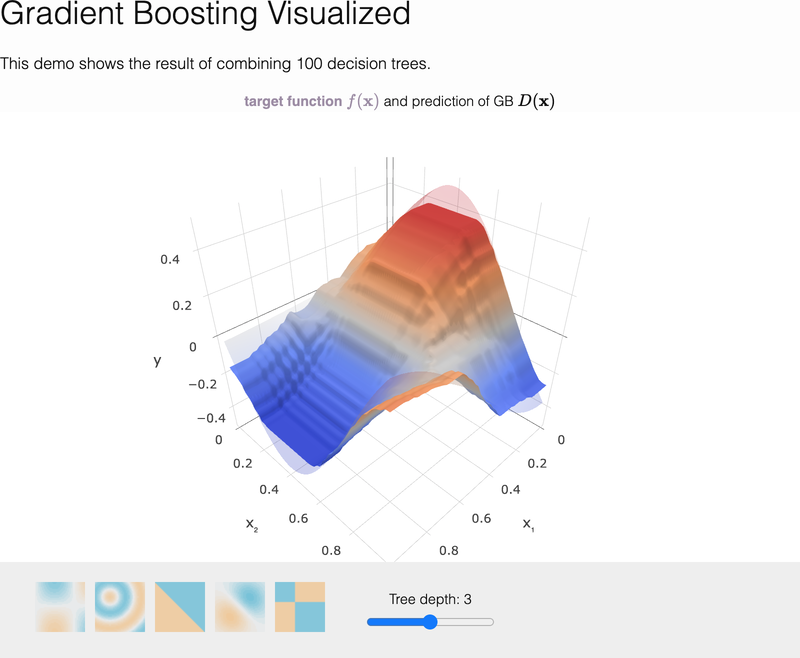
\includegraphics[width=0.93\linewidth]{images/supervised/z_algorithms_ensemble/gradient_boosting_depth_3.png}
%			\caption{}
		\end{figure}
	\end{columns}
	
	\begin{center}
		Prova la demo live al seguente link: \underline{\href{http://arogozhnikov.github.io/2016/06/24/gradient_boosting_explained.html}{Gradient Boosting explained}}
	\end{center}
	
\end{frame}


\begin{frame}
	
	\frametitle{Decision Tree vs Gradient Boosting: depth 6}

	\begin{columns}
		\column{0.50\linewidth}
		\begin{figure}[!htbp]
			\centering
			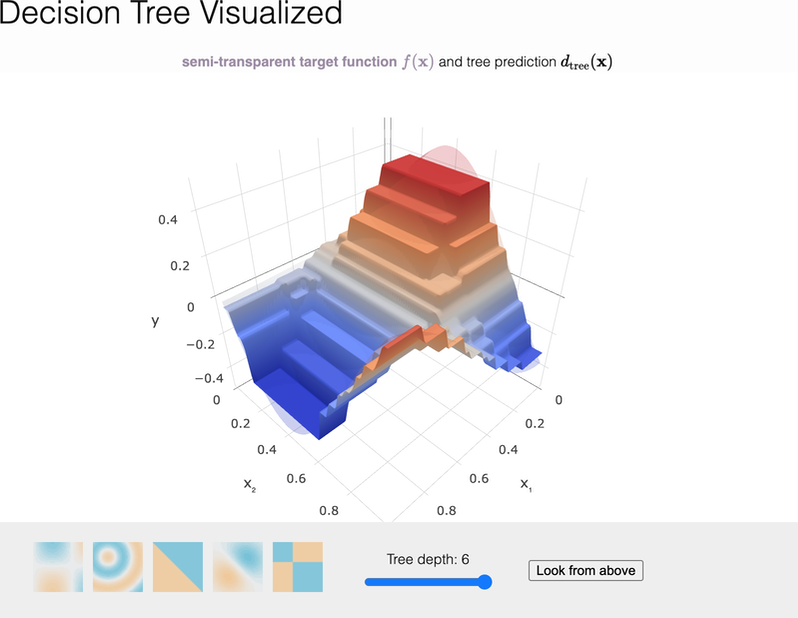
\includegraphics[width=1.0\linewidth]{images/supervised/z_algorithms_ensemble/decision_tree_depth_6.png}
%			\caption{}
		\end{figure}
		
		\column{0.50\linewidth}
		\begin{figure}[!htbp]
			\centering
			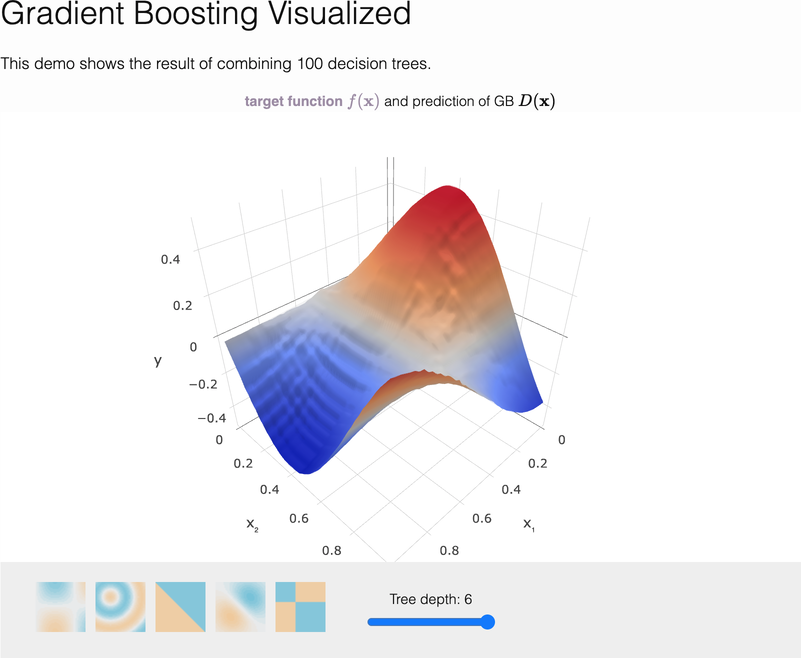
\includegraphics[width=0.93\linewidth]{images/supervised/z_algorithms_ensemble/gradient_boosting_depth_6.png}
%			\caption{}
		\end{figure}
	\end{columns}
	
	\begin{center}
		Prova la demo live al seguente link: \underline{\href{http://arogozhnikov.github.io/2016/06/24/gradient_boosting_explained.html}{Gradient Boosting explained}}
	\end{center}
	
\end{frame}